\subsection{Bazinė CNN modelio klasė}
\label{subsec:base_cnn}

Klasė \texttt{BaseCNN} aprašo bendrą konvoliucinio tinklo šabloną – iš jos paveldi \texttt{ImageCNN} (su \texttt{nn.Conv2d}) ir \texttt{KeystrokeCNN} (su \texttt{nn.Conv1d}). Paveldinčios klasės nurodo tik konvoliucinių, telkimo ir paketinio normalizavimo sluoksnių dimensijas (žr.~\ref{fig:base_cnn_class} pav.).

\begin{figure}[H]
    \centering
    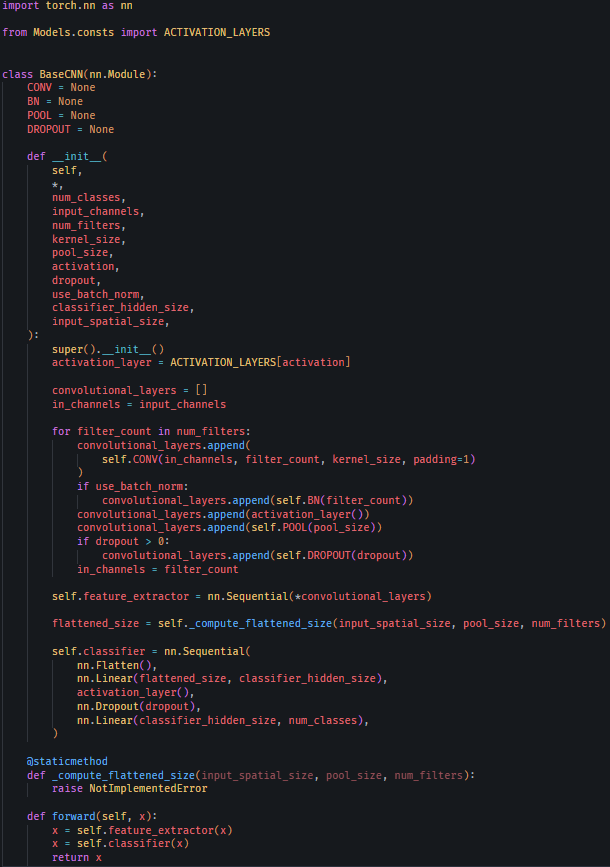
\includegraphics[width=0.85\linewidth]{3Lab/overleaf/images/BaseCNN_Class.png}
    \caption{Bazinės CNN modelio klasės kodas.}
    \label{fig:base_cnn_class}
\end{figure}

Tinklo struktūros komponentai:
\begin{itemize}
    \item \textbf{Konvoliucinis sluoksnis} (\texttt{CONV}) – išmoksta lokalius požymius (briaunos, formos vaizdams; laikinės šablonų formos požymiai laiko eilutėms). \texttt{padding}~$=1$ išlaiko erdvinę dimensiją iki telkimo.
    \item \textbf{Paketinis normalizavimas} (\texttt{BN}) – stabilizuoja tarpinių aktyvavimų pasiskirstymą, leidžia naudoti didesnį mokymosi greitį ir veikia kaip silpnas reguliarizatorius.
    \item \textbf{Aktyvacijos funkcija} – įveda netiesiškumą; konfigūruojama per \texttt{ActivationFunction} enumeraciją (\textit{ReLU}, \textit{LeakyReLU}, \textit{Tanh}, \textit{ELU}, \textit{Sigmoid}).
    \item \textbf{Telkimo sluoksnis} (\texttt{POOL}) – sumažina erdvinę dimensiją perpus, taip didindamas receptyvinį lauką ir mažindamas skaičiavimo kaštus.
    \item \textbf{\textit{Dropout}} – atsitiktinai išjungia dalį neuronų, kovoja su persimokymu (\textit{overfitting}).
    \item \textbf{Klasifikatorius} – \texttt{Flatten}~$\rightarrow$ paslėptas pilnai sujungtas sluoksnis su aktyvacija ir \textit{Dropout}~$\rightarrow$ išėjimo sluoksnis su tiek neuronų, kiek yra klasių (raw \textit{logits}, \texttt{Softmax} įjungiamas \texttt{CrossEntropyLoss} viduje).
\end{itemize}

Mokymo eiga:
\begin{itemize}
    \item Pirmyninis žingsnis (\texttt{forward}): įėjimas paeiliui pereina visus konvoliucinius blokus ir klasifikatorių, gaunami $C$ \textit{logits} reikšmių vektoriai, kur $C$ – klasių skaičius.
    \item Atgalinis žingsnis: \texttt{loss.backward()} per \texttt{autograd} mechanizmą apskaičiuoja kiekvieno svorio gradientą; \texttt{optimizer.step()} atnaujina svorius pagal pasirinktą algoritmą (\textit{Adam}, \textit{AdamW}, \textit{RMSprop} arba \textit{SGD}).
\end{itemize}

Klasės kodas parašytas autoriaus. \texttt{nn.Sequential} grandinės sukomponavimo pavyzdžiai paimti iš \texttt{PyTorch} oficialaus mokymo kodo.
